\section{Information page}
\subsection*{Students}
\begin{tabular}{ll}
   & Arponen Jani \\
   & Ogenda Dancun \\
   & Ruley Brian \\
   & Varis Leo \\
\end{tabular}

\subsection*{Official Instructor}
\begin{tabular}{ll}
   & Sarolahti Pasi \\
\end{tabular}


% \subsection*{Approval}
% The Instructor has accepted the final version of this document
% Date: xx.2.2020

\subsection*{Changelog}
\begin{table}[!h]
\small{
\begin{tabular}{l|l|l|l}
\textbf{Version} & \textbf{Date} & \textbf{Author} & \textbf{Description} \\
\hline
0.1 & 2020-08-26 & All & Template \\
0.9 & 2020-08-27 & Jani & Majority written. TODO: Dancun info on GUI.\\
0.9.1 & 2020-08-27 & Jani & Requirement B5 was implemented, changed to Yes \\ 
\end{tabular}
}
\caption{Document changelog.}
\label{table:changelog}
\end{table}


\newpage 
\tableofcontents

\newpage
\section{Introduction} 

The purpose of this document is to be the final documentation of the project in the \textit{ELEC-A7151 - Object oriented programming with C++} course. The output of the project was a network simulator  where it is possible to build simple networks and simulate traffic between nodes. The project plan outlined the features that we aimed to implement:

\begin{table}[!htbp]
\footnotesize{
\begin{tabular}{p{0.11\textwidth}|p{0.06\textwidth}|p{0.6\textwidth}|p{0.11\textwidth}}
\textbf{Module} & \textbf{Req\#} & \textbf{Requirement} & \textbf{Implemented} \\
\hline Compatibility
& S1        & It shall be possible to compile and run the program on Ubuntu 18.04. & Yes\\
& S2        & A CMake file shall be provided together with the source code upon completion. & Yes\\
\hline Network model   
& B1        & The network shall be modeled by nodes and links between nodes. Communication between nodes shall be done by (data) packets over the links.  & Yes \\
& B1.1      & Links shall be defined by a transmission speed and a propagation delay, which shall govern: 1. how fast new packets can be sent; and 2. how fast they propagate over the link. There shall be a way to queue packets at the node before the link. & Yes \\
& B1.2      & Nodes shall be defined by an address and are of a type: router or end-host. & Yes\\
& B1.2.1    & Routers shall be able to route packets between other nodes. & Yes\\
& B1.2.2    & End-hosts shall be able to run applications that can send and/or receive packets to/from other end-hosts for a specified length of time. & Yes\footnote{}\\
& B2        & The model code shall be written in such a way that it is easy to extend with e.g. new kinds of links or applications. & Yes\\ 
\hline Program
& B3        & Running simulations shall be "easily configurable" for different network scenarios, through e.g. configuration files. & \textcolor{red}{TODO}\\
& B4        & It shall be possible to collect statistics on the simulated network, e.g. packet to destination times, link utilization, queue lengths, etc. & No\\
& B5        & From the applications user interface, it shall be possible to follow the progress of simulation, including statistics and states for links, queues and packets. & Yes \\
\hline GUI
& A1        & There shall be a graphical user interface (GUI) for the program to interact with all other functionalities. & No\\
& A1.1      & B5 shall be expanded to an animation on the GUI. & No\\
\hline Expanded functionality
& A2        & B1.1 shall be expanded to create different queue behaviours, including limited queues and as a result, dropped packets. & No\\
& A3        & B1.1 and B1.2 shall be expanded to include mobile hosts, i.e. wireless links. & No\\
& A3.1      & Communication parameters of wireless links shall be defined by signal strength. & No\\
& A3.2      & Mobile hosts shall be able to move around in a 2D map with obstacles that reduce the signal strength of the wireless link. & No\\
\hline
\end{tabular}
}
\caption{The programs functional requirements and implementation status. (1: Only one application was implemented.) }
\label{table:requirements}
\end{table}

\section{Software structure}
The architecture is very straight forward and shown in figure \ref{img:classdiagram}. Note that the diagram doesn't show absolutely everything, e.g. some getters and setters are excluded together with unimportant data types and some helper methods. An explanation of each classes role in the architecture follows below. 
\\\\
The root class is \texttt{Simulatable}, which handles the simulations timesteps through \texttt{evt\_times[]} and \texttt{AdvanceTime()}. Each simulatable point in the inherited classes has an entry in \texttt{evt\_times[]}, which basically determines how many timesteps to go until it can be executed. A value of -1 indicates nothing to simulate and once every \texttt{evt\_times[]} entry of every \texttt{Simulatable} is equal to -1, the simulations is ran.
\\\\
The \texttt{NetworkInterface} class handles the IP address and every \texttt{Node} holds one. Initially the plan was for a node to be able to hold multiple network interfaces and a full LAN / WAN implementation for routing packets.
\\\\
The \texttt{Packet} class is an arbitrarily simplified TCP packet, holding the important (to our simulation) headers, such as source and target addresses and a time-to-live value, which gets reduced by 1 on each routing event.
\\\\
The \texttt{Node} class inherits from \texttt{Simulatable} and has multiple functions. For instance, it holds a reference to all neighboring nodes and which links are used to connect to those in the \texttt{connected[]} variable. Packets are handled in separate \texttt{receive[]} and \texttt{transmit[]} queues, the latter of which also holds a reference to which currently connected node the packet is to be transferred to. Multiple helper methods exist, e.g. for connecting or disconnecting from neighboring nodes and moving packets. The \texttt{RunApplication()} method is overloaded by inherited classes to implement application specific functionality.
\\\\
The \texttt{Link} class inherits from \texttt{Simulatable} and is used to link nodes together. The main parameters are \texttt{transmissionspeed} and \texttt{propagationdelay}, which ultimately result in the timestamp written back to \texttt{Simulatable.evt\_times[]}. The link also holds two \texttt{transmissionqueue} variables, which are the currently in transfer packets.
\\\\
The \texttt{EndHost} class inherits from \texttt{Node} and is the node that ultimately generates packets that will be sent to another endhost. The implemented functionality simply generates random sized packets (amount equal to \texttt{packetcount}) with the specified \texttt{targetadr}. If the target address is set to self (as it is by default) then no packets are generated. 
\\\\
The \texttt{Router} class inherits from \texttt{Node} and is the node responsible for routing packets between other nodes. The way this is done, is by going through the \texttt{Node.receive} queue and looking up the self, target address in a routing table generated by the \texttt{Network}. If no route exists, the packet is dropped.
\\\\
The \texttt{Network} class ties everything else together. It is the interface to creating and removing nodes, linking and unlinking them and other graph behaviour. The \texttt{routingtable} map is generated by running Dijkstra's shortest path algorithm from every source node to every target node. The \texttt{Network} also holds the functionality to \texttt{Save} and \texttt{Load} JSON files which contain the network configuration.

\begin{figure}[!htbp]
\begin{center}
	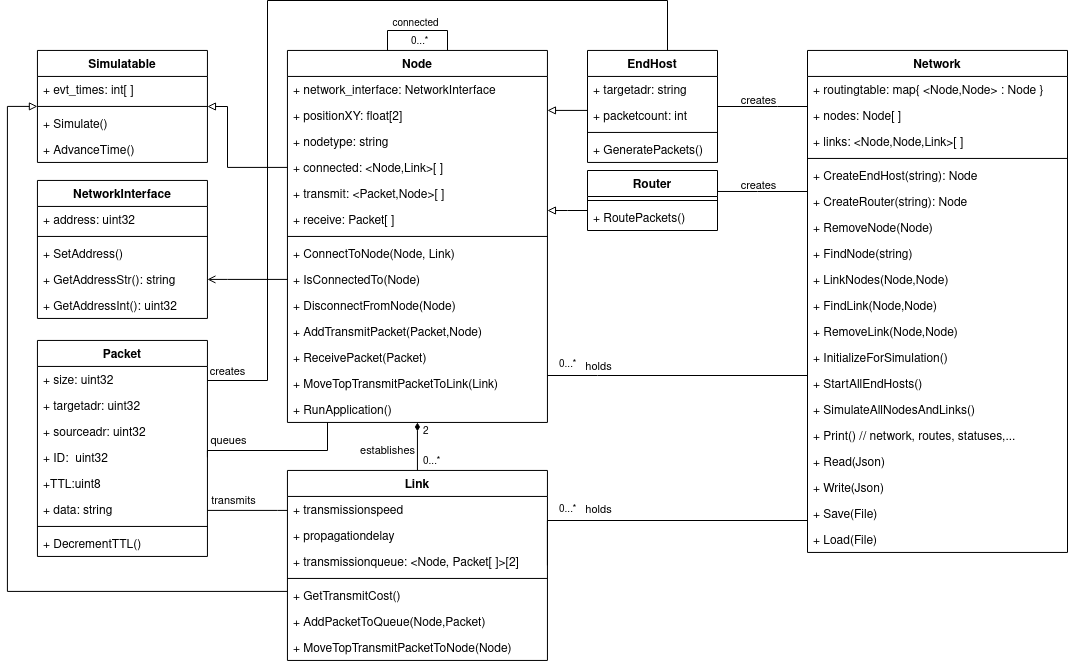
\includegraphics[width=13cm]{classdiagrams.png}
    \caption{Network simulator class diagrams.}
	\label{img:classdiagram}			% use \ref{img:example} to refer to this figure
\end{center}
\end{figure}

\section{Build instructions}
\begin{enumerate}
    \item Clone the project repository to your machine, or download and unzip.
    \item Open terminal and navigate to the project root, run \texttt{cd src/nwsim}
    \item Build the software by first generating the Makefile with \texttt{cmake CMakeLists.txt} and then running \texttt{make}
    \item The software is built to the projects root/bin and the executables name is \texttt{nwsim-cli}
\end{enumerate}

\section{Running the software}
The software is a CLI implementation and has rather intuitive usage. For usage, please run the \texttt{help} command, or see the compiled version below in section \ref{sec:help}.

\subsection{Example on running the simulator}
\begin{enumerate}
    \item Open a terminal and navigate to the project root. Run the simulator with \texttt{./bin/nwsim-cli}
    \item At any point, type \texttt{help} for usage.
    \item Create an endhost node with \texttt{add e 1.1.1.1}, you will enter edit mode for this node:
    \begin{enumerate}
        \item Run \texttt{list} to see all changeable parameters.
        \item \texttt{exit} or \texttt{quit} or \texttt{q} to drop out of editmode.
    \end{enumerate}
    \item Create a router node with \texttt{add r 2.2.2.2}, drop out of editmode.
    \item Create another endhost node with \texttt{add e 3.3.3.3}, in editmode configure:
    \begin{enumerate}
        \item \texttt{set target 1.1.1.1} to set target to the first endhost.
        \item \texttt{set count 100} to send 100 packets from this endhost.
    \end{enumerate}
    \item Edit the first endhost with \texttt{edit 1.1.1.1} and configure:
    \begin{enumerate}
        \item \texttt{set target 3.3.3.3}
        \item \texttt{set count 50}
    \end{enumerate}
    \item Link the first endhost to the router with \texttt{link 1.1.1.1 2.2.2.2}, and enter links editmode:
    \begin{enumerate}
        \item Run \texttt{list} to see all changeable parameters.
        \item \texttt{set ts 100} to set transmission speed to 100 timeunits.
        \item \texttt{set pd 2} to set propagation delay to 2 timeunits / byte.
        \item \texttt{exit} or \texttt{quit} or \texttt{q} to drop out of editmode.
    \end{enumerate}
    \item To finish the network, link the remaining endhost and the router \texttt{link 2.2.2.2 3.3.3.3} and configure:
    \begin{enumerate}
        \item \texttt{set ts 50} 
    \end{enumerate}
    \item If you created unnecessary nodes, they can be removed with \texttt{rem <adr>}
    \item If you linked the wrong nodes, they can be disconnected with \texttt{unlink <adr> <adr>}
    \item If you wish to edit the links parameters, run \texttt{edit <adr> <adr>}
    \item Run \texttt{list} to see the current network configuration.
    \item Enter the simulation mode with \texttt{sim}
    \begin{enumerate}
        \item Run \texttt{list} to see all endhosts that will be sending packets during the simulation.
        \item Run \texttt{routes} to see the routing table and check that your network isn't missing a crucial link.
        \item Start the simulation with the \texttt{run} command. You will go back to the simulation mode once the simulation has finished.
        \item To exit simulation mode, use \texttt{exit} or \texttt{quit} or \texttt{q}
    \end{enumerate}
    \item To save the current network configuration, run \texttt{save <filename>}
    \item To load a new network configuration from a file, run \texttt{load <filename>}, NOTE: this will overwrite the current configuration.
    \item To exit the program, use \texttt{exit}
\end{enumerate}

\subsection{Help documentation} \label{sec:help}
\lstset{basicstyle=\scriptsize}
\begin{lstlisting}
LEGEND:
<mode>      - edit, sim
<filename>  - JSON file to save/load network config
<adr>       - IP address in octet format, e.g. 192.168.0.1
<int>       - integer, note that parameters are capped between valid values.
NWSIM HELP:
help                - Print this manual.
       <mode>       - Prints mode specific usage.
save   <filename>   - Save current network configuration as JSON to given file.
load   <filename>   - Discard current network configuration and load from specified file.
exit                - Exit current mode or if at root, exits the program.
list                - Lists all current nodes and what other nodes they are linked to.
add    e|r <adr>    - Adds an [e]ndhost or [r]outer with given address.
                      NOTE: Address must be IP format and unique in network.
rem    <adr>        - Removes an endhost or router that matches the given address, and
                      severs affected links. If node doesn't exist, nothing happens.
link   <adr> <adr>  - Links given nodes, if they exist.
unlink <adr> <adr>  - Unlinks given nodes, if they are currently linked.
edit   <adr>        - Enter node (endhost, router) edit mode.
edit   <adr> <adr>  - Enter link edit mode.
sim                 - Enter simulation mode.
tests               - Prinst result of all tests and exit program.
EDIT MODE HELP:
help                - Print this help for edit mode.
exit                - Exit edit mode.
list                - List all changeable parameters.
NODE SPECIFIC EDIT MODE HELP:
set   address <adr> - Changes this nodes to use the given address.
                      NOTE: Address must be IP format and unique in network.
ENDHOST SPECIFIC EDIT MODDE HELP:
set target <adr>    - Requires endhost source and endhost target. Sets target address.
                      NOTE: Address must be IP format and exist in current network.
                            If set to self, no packets sent in simulation.
set count <int>     - Requires endhost. Sets amount of packets sent to target.
LINK SPECIFIC EDIT MODE HELP:
set ts <int>        - Sets links transmission speed to given value (timeunit). Value 
                      determines the interval at which new packets can be transmitted
                      to the link.
set pd <int>        - Sets links propagation delay to given value (timeunit / byte).
                      Value determines the time it takes for a packet to travel across
                      the link. time = propagation_delay * packet_size
SIM MODE HELP:
help                - Print this help for sim mode.
list                - Lists all endhosts that are configured to send packets.
routes              - Prints current network routing table.
run                 - Starts simulation.
\end{lstlisting}

\section{Tests}
The software was tested while it was being written and refactored, by writing unit tests and updating as necessary when the underlying logic changed. The \texttt{src/nwsim/tests/testroutines.hpp} file holds all testcases and they can be executed in software by running the \texttt{tests} command. The program output was then simply searched for the flag \texttt{false} for any tests that didnt pass, e.g:
\begin{enumerate}
    \item \texttt{./bin/nwsim-cli | tee testout.txt}
    \item Run the \texttt{tests} command for test output and \texttt{exit}
    \item Search for tests that didnt pass with \texttt{grep false testout.txt}
\end{enumerate}

\subsection{Test output}
Below is the output of running \texttt{tests} in the program. Note that all tests that pass hold value \texttt{true}. If it was not possible to write simple and quick enough tests, e.g. for the routing table or actual simulation output, then a manual look is needed.
\\\\
Note in the simulation test output not all packets have moved to their corresponding nodes. This is because the test is only run for \texttt{n} timesteps, and the packet counts are too high to be transferred during this,

\lstset{basicstyle=\scriptsize}
\begin{lstlisting}
==============================
TESTING - NWSim::Packet class
==============================

Default constructed packet should have:
	ttl = 0: true
	decrementing ttl is still 0: true
	target address all zeroes: true
	source address all zeroes: true
	ID = 0: true
	data string is empty: true
	size = MINPACKETSIZE: true
	can set size to >= MINPACKETSIZE: set to 123: true
	can NOT set size to < MINPACKETSIZE: set to 0, size now: 18
Using "actual" constructor with valid data:
data = test, target = 123.123.123.123, source = 255.255.255.255, ID = 666
	ttl = 255: 255
	decrementing ttl gives 254: true
	target address matches: true
	source address matches: true
	ID matches: true
id is666should be666
	data string is test: true
	size is MINPACKETSIZE + len(test): true

==============================
TESTING - NWSim::Address helpers
==============================

Converting from int to string:
	arg 0 gives 0.0.0.0: true
	UINT32_MAX gives 255.255.255.255: true
Converting from str to int:
	0.0.0.0 = 0: true
	255.255.255.255 = UINT32_MAX: true
	Testing randomly generated (valid) address strings:: 
		Generated str '3.182.89.53' doesnt throw - : true
		Generated str '31.253.46.58' doesnt throw - : true
		Generated str '1.134.129.19' doesnt throw - : true
		Generated str '95.167.144.3' doesnt throw - : true
		Generated str '180.3.111.222' doesnt throw - : true
		Generated str '100.172.49.85' doesnt throw - : true
		Generated str '101.153.212.37' doesnt throw - : true
		Generated str '151.240.19.26' doesnt throw - : true
		Generated str '39.108.206.70' doesnt throw - : true
		Generated str '106.252.1.234' doesnt throw - : true
		Generated str '3.130.254.99' doesnt throw - : true
	invalid address "asd" throws: true
	invalid address "1" throws: true
	invalid address "255.255.255.256" throws: true
Double wrapped:
	Setting to 1.2.3.4, converting to int, and back to str, matches: true

==============================
TESTING - NWSim::NetworkInterface class
==============================

NOTE: Valid addresses handled by NWSim::Address helpers!
Default constructed
	address is 0: true
	Possible to set address to valid one 1.2.3.4: true
	Address string matches after setting: true
	NOT Possible to set address to invalid one invalid adr: true
	Address string hasn't changed after setting to invalid: true
adr should be 1.2.3.41.2.3.4
Constructing with given VALID adr '1.2.3.4'
	Address string matches after constructing: true
Constructing with given INVALID adr 'invalid adr'
	Address string should be 0.0.0.0 after constructing: true

==============================
TESTING - NWSim::Node class
==============================

NOTE: Addressing handled by NWSim::NetworkInterface!
NOTE: Methods that cannot be tested without network/link:
	ConnectToNode,IsConnectedTo,DisconnectFromNode,MoveTopTransmitPacketToLinkRunApplication: 
Can generate default constructed nodes:
	Default pos is (0,0): true
	Can move to new position (1.2,3.4): true
	Node type is "DEFAULT": true
	NOT connected to any other nodes: true
	Transmit queue is empty: true
	Receive queue is empty: true
	Default address is 0.0.0.0: true
Using "correct" constructor:
	Constructed at pos (1.200000,3.400000): true
	Constructed with adr 1.2.3.4: true
Compare node equality (address):
	Node against same adr as str: true
	Two different nodes with different IP's are NOT the same: true
	Comparing node to itself is equal: true
Packet handling of the Node
	After receiving 1 packet, receive queue holds 1 packet: : true
	Can NOT add packet with TTL==0 to transmit queue: : true
	Can add packet with TTL>0 to transmit queue: : true

==============================
TESTING - NWSim::EndHost class
==============================

NOTE: Only checking EndHost specific functionality, check Node for shared, or Network for "fuller" functions.
Packet generation variables
	Node type is EndHost: true
	Initial packet count is MINPACKETS: true
	Can set packet count >MINPACKETS but <= MAXPACKETS: true
	Can NOT set packet count >MAXPACKETS, clamped to MAXPACKETS: true
	Initial target address is self: true
	Can set target address to a new valid one: true
	Target address after set matches: true
	Can NOT set target address to a new invalid one: true
	Target address after ivnalid set  matches old one: true

==============================
TESTING - NWSim::Router class
==============================

NONE YET, TODO, false
Default constructor
	Node type is Router: true

==============================
TESTING - NWSim::Link class
==============================

NOTE: Methods that cannot be tested without network/link:
	InitTransmissionQueues,MoveTopTransmitPacketToNode,AddPacketToQueue: 
Default constructed:
	transmission speed is MIN: true
	propagation delay is MIN: true
	transmission speed is set: true
	propagation delay is set: true
Constructed with 0,0:
	transmission speed is MIN: true
	propagation delay is MIN: true
Constructed with 123,321:
	transmission speed is 123: true
	propagation delay is 321: true

==============================
TESTING - NWSim::Network class
==============================

NOTE: A deeper exploration of node/link specific functions in their respective tests.
Empty network tests
	New network is empty: true
	A non-existent node can not be found and returns nullptr: true
	Can add default EndHost: true
	Can find existing node: true
	Can NOT add node with same IP again: true
Linking nodes...
	After adding another host and router, size is 3: true
	Linking two nodes worked: true
	Attempting to relink throws an exception: true
	Attempting to backwards relink throws an exception: true
	Linking other two nodes worked: true
Removing node from network
	Network size is 2 nodes: true
	Removing the router between hosts severed all links: ...
		h1 -/- r1: true
		h2 -/- r1: true
		h1 size == 0: true
		h2 size == 0: true
Removing link from network
	Network size is 3 as no nodes removed: true
	Removing a link between h1,r2 only removes that link: ...
		h1 -/- r2: true
		h2 --- r2: true
		h1 size == 0: true
		h2 size == 1: true
**** Manually see below routing table if it makes sense... ****
	New print table should not be simulatable out of the box: true
Current routing table size: 9
	When at: 0.0.0.11	and target: 0.0.0.22	send to: 0.0.0.22
	When at: 0.0.0.11	and target: 0.0.0.33	send to: 0.0.0.22
	When at: 0.0.0.22	and target: 0.0.0.11	send to: 0.0.0.11
	When at: 0.0.0.22	and target: 0.0.0.33	send to: 0.0.0.33
	When at: 0.0.0.33	and target: 0.0.0.11	send to: 0.0.0.22
	When at: 0.0.0.33	and target: 0.0.0.22	send to: 0.0.0.22
Testing packet transfer in network
	Setting target adr for h1: true
	Before run, transmit queue size is 0: true
	After run transmit queue == packetcount == set packet count: true
Starting packet movement...
	Link is empty and can not move any packets: true
	Moving packet from node h1 to link is succesful: true
	Link h1-r1 now has 1 packet: true
	Link has moved packet to next node r1: true
	Next link l1 timestamp should be 0 as no other packets exist: true
	After running router, receive queue is 0 and transmit is 1: true
	After moving from the router, transmit q is empty: true
	Link has moved packet to next node h2: true
	Next link l2 timestamp should be 0 as no other packets exist: true
Moving the remaining packets...
	Before run - h1 and l1 are empty: true
	Before run - Router reveived holds rest of the packets: true
Source: 0.0.0.11	Target: 0.0.0.33	Size: 30	TTL: 255	ID: 1	Data: Test
Source: 0.0.0.11	Target: 0.0.0.33	Size: 29	TTL: 255	ID: 2	Data: Test
Source: 0.0.0.11	Target: 0.0.0.33	Size: 22	TTL: 255	ID: 3	Data: Test
Source: 0.0.0.11	Target: 0.0.0.33	Size: 40	TTL: 255	ID: 4	Data: Test
	After run - Router transmit holds rest of the packets: true
	All packets found on endhost: true
Source: 0.0.0.11	Target: 0.0.0.33	Size: 41	TTL: 254	ID: 0	Data: Test
Source: 0.0.0.11	Target: 0.0.0.33	Size: 30	TTL: 254	ID: 1	Data: Test
Source: 0.0.0.11	Target: 0.0.0.33	Size: 29	TTL: 254	ID: 2	Data: Test
Source: 0.0.0.11	Target: 0.0.0.33	Size: 22	TTL: 254	ID: 3	Data: Test
Source: 0.0.0.11	Target: 0.0.0.33	Size: 40	TTL: 254	ID: 4	Data: Test
**** Testing Simulatable runs ****
	Set up network, can not run yet: true
	Initialized network for running: true
	Check below routing table...: 
Current routing table size: 25
	When at: 1.1.1.1	and target: 2.2.2.2	send to: 3.3.3.3
	When at: 1.1.1.1	and target: 3.3.3.3	send to: 3.3.3.3
	When at: 1.1.1.1	and target: 4.4.4.4	send to: 3.3.3.3
	When at: 1.1.1.1	and target: 5.5.5.5	send to: 3.3.3.3
	When at: 2.2.2.2	and target: 1.1.1.1	send to: 3.3.3.3
	When at: 2.2.2.2	and target: 3.3.3.3	send to: 3.3.3.3
	When at: 2.2.2.2	and target: 4.4.4.4	send to: 3.3.3.3
	When at: 2.2.2.2	and target: 5.5.5.5	send to: 3.3.3.3
	When at: 3.3.3.3	and target: 1.1.1.1	send to: 1.1.1.1
	When at: 3.3.3.3	and target: 2.2.2.2	send to: 2.2.2.2
	When at: 3.3.3.3	and target: 4.4.4.4	send to: 4.4.4.4
	When at: 3.3.3.3	and target: 5.5.5.5	send to: 4.4.4.4
	When at: 4.4.4.4	and target: 1.1.1.1	send to: 3.3.3.3
	When at: 4.4.4.4	and target: 2.2.2.2	send to: 3.3.3.3
	When at: 4.4.4.4	and target: 3.3.3.3	send to: 3.3.3.3
	When at: 4.4.4.4	and target: 5.5.5.5	send to: 5.5.5.5
	When at: 5.5.5.5	and target: 1.1.1.1	send to: 4.4.4.4
	When at: 5.5.5.5	and target: 2.2.2.2	send to: 4.4.4.4
	When at: 5.5.5.5	and target: 3.3.3.3	send to: 4.4.4.4
	When at: 5.5.5.5	and target: 4.4.4.4	send to: 4.4.4.4
Actual simulation ---
Packet counts before simulation:
EndHost 1.1.1.1          - transmit: 100    receive: 0     
EndHost 2.2.2.2          - transmit: 50     receive: 0     
Router  3.3.3.3          - transmit: 0      receive: 0     
Router  4.4.4.4          - transmit: 0      receive: 0     
EndHost 5.5.5.5          - transmit: 10     receive: 0     
Packet counts after simulation:
1.1.1.1          - 3.3.3.3          : 85    waiting: (  -1,4)
2.2.2.2          - 3.3.3.3          : 33    waiting: (  -1,19)
3.3.3.3          - 4.4.4.4          : 17    waiting: (  -1,9)
4.4.4.4          - 5.5.5.5          : 1     waiting: (  -1,9)
EndHost 1.1.1.1          - transmit: 0      receive: 10    
EndHost 2.2.2.2          - transmit: 0      receive: 0     
Router  3.3.3.3          - transmit: 0      receive: 0     
Router  4.4.4.4          - transmit: 0      receive: 0     
EndHost 5.5.5.5          - transmit: 0      receive: 14   
\end{lstlisting}

\section{Work log}
The amount of hours for each week for every group member is described here.

\begin{table}[!htbp]
\footnotesize{
\begin{tabular}{c|p{0.15\textwidth}|c|p{0.55\textwidth}}
\textbf{Week} & \textbf{Dates} & \textbf{Hours} & \textbf{What was done?} \\
\hline 1 & July 6 - July 12     & 2 & Project plan \\
\hline 2 & July 13 - July 19    & 3 & Weekly meeting, node, link and network design. \\
\hline 3 & July 20 - July 26    & 11 & Weekly meeting, studying CMake and Qt Creator. initial work on IP address handling helpers, NetworkInterface, Packet, Node, Link and Application classes. Test cases for NetworkInterface and Packet.  \\
\hline 4 & July 27 - Aug 2      & 6 & Weekly meeting. Continued work on Node and Link classes. Tests for Nodes, Links and initial packet transfer. Node position variables + tests for Dancun. \\
\hline 5 & Aug 3 - Aug 9        & 2 & Weekly meeting. Mid-term meeting with Pasi. \\
\hline 6 & Aug 10 - Aug 16      & 0 & Nothing \\
\hline 7 & Aug 17 - Aug 23      & 25 & Weekly meeting. Major refactor and cleanup of Node and Link classes, dropped Application as a separate class. Network class to hold Nodes and Links, routing, EndHost, Router, Packet generation. Testcases for Node, Link, Network. Moved testcases to separate file and introduced assert checks to grep for fails.  \\
\hline 8 & Aug 24 - Aug 30      & 30 & Weekly meeting. Simulatable nodes and links, packet transfer between them, fix routing, testcases. Wrote CLI as GUI was abandoned. Final documentation. Reviewing file save/load implementation from Brian. \\
\hline\hline\textbf{Total}&All  & 79 & - \\
\end{tabular}
}
\caption{Jani's work log. Hours are rough estimates from git commit history, stopped tracking on week 7 to keep up.}
\label{table:worklog-jani}
\end{table}

%TODO: Dancun
\begin{table}[!htbp]
\footnotesize{
\begin{tabular}{c|p{0.15\textwidth}|c|p{0.55\textwidth}}
\textbf{Week} & \textbf{Dates} & \textbf{Hours} & \textbf{What was done?} \\
\hline 1 & July 6 - July 12     & 0 & Something or nothing \\
\hline 2 & July 13 - July 19    & 0 & Something or nothing \\
\hline 3 & July 20 - July 26    & 0 & Something or nothing \\
\hline 4 & July 27 - Aug 2      & 0 & Something or nothing \\
\hline 5 & Aug 3 - Aug 9        & 0 & Something or nothing \\
\hline 6 & Aug 10 - Aug 16      & 0 & Something or nothing \\
\hline 7 & Aug 17 - Aug 23      & 0 & Something or nothing \\
\hline 8 & Aug 24 - Aug 30      & 0 & Something or nothing \\
\hline\hline\textbf{Total}&All  & 0 & - \\
\end{tabular}
}
\caption{Dancun's work log. }
\label{table:worklog-dancun}
\end{table}

%TODO: Brian
\begin{table}[!htbp]
\footnotesize{
\begin{tabular}{c|p{0.15\textwidth}|c|p{0.55\textwidth}}
\textbf{Week} & \textbf{Dates} & \textbf{Hours} & \textbf{What was done?} \\
\hline 1 & July 6 - July 12     & 0 & Something or nothing \\
\hline 2 & July 13 - July 19    & 0 & Something or nothing \\
\hline 3 & July 20 - July 26    & 0 & Something or nothing \\
\hline 4 & July 27 - Aug 2      & 0 & Something or nothing \\
\hline 5 & Aug 3 - Aug 9        & 0 & Something or nothing \\
\hline 6 & Aug 10 - Aug 16      & 0 & Something or nothing \\
\hline 7 & Aug 17 - Aug 23      & 0 & Something or nothing \\
\hline 8 & Aug 24 - Aug 30      & 0 & Something or nothing \\
\hline\hline\textbf{Total}&All  & 0 & - \\
\end{tabular}
}
\caption{Brian's work log. }
\label{table:worklog-brian}
\end{table}

\begin{table}[!htbp]
\footnotesize{
\begin{tabular}{c|p{0.15\textwidth}|c|p{0.55\textwidth}}
\textbf{Week} & \textbf{Dates} & \textbf{Hours} & \textbf{What was done?} \\
\hline 1 & July 6 - July 12     & 1 & Project plan \\
\hline 2 & July 13 - July 19    & 2 & Attended weekly meeting, planned parts of the implementation \\
\hline 3 & July 20 - July 26    & 2 & Attended weekly meeting, wrote initial version of event queue \\
\hline 4 & July 27 - Aug 2      & 2 & Attended weekly meeting, rewrote event queue \\
\hline 5 & Aug 3 - Aug 9        & 1 & Attended weekly meeting \\
\hline 6 & Aug 10 - Aug 16      & 1 & Attended weekly meeting \\
\hline 7 & Aug 17 - Aug 23      & 3 & Attended weekly meeting, created routing table for the network \\
\hline 8 & Aug 24 - Aug 30      & 0 & nothing \\
\hline\hline\textbf{Total}&All  & 12 & - \\
\end{tabular}
}
\caption{Leo's work log. }
\label{table:worklog-leo}
\end{table}
\hfill
\section{Post mortem}
It is quite obvious from the output of the project that we did not meet the goal that we set for ourselves and what was expected from the project description. There are many reasons for why this was the case, but the core issues were:
\begin{enumerate}
    \item Work was probably divided wrong from the start, e.g. Jani had work until the last 2 weeks of the project, but everyone else was waiting for the results of his code. Similarly, Leo had free time at the start, but less towards the end. See figure \ref{img:schedule} for the original schedule from the project plan.
    \item Design of the software was only done superficially and at a too high level. The approach was to design further as we progressed, but this turned out to be a bad decision. Ad-hoc approach to design rarely works, and here it didn't either.
    \item Related to the design, but the architecture was started from the bottom up, which introduced some unnecessary issues, which could have been averted if the network was immediately designed as a graph and the necessary interfaces implemented early, such that other group members wouldn't have to worry about ever-changing code.
    \item The GUI portion was started early and progressed fine, but it was never properly integrated with the core functionality. This is why, in the end, a CLI approach was taken as there was not enough time left to write a shorter implementation and integration. 
\end{enumerate}

\begin{figure}[!htbp]
\begin{center}
	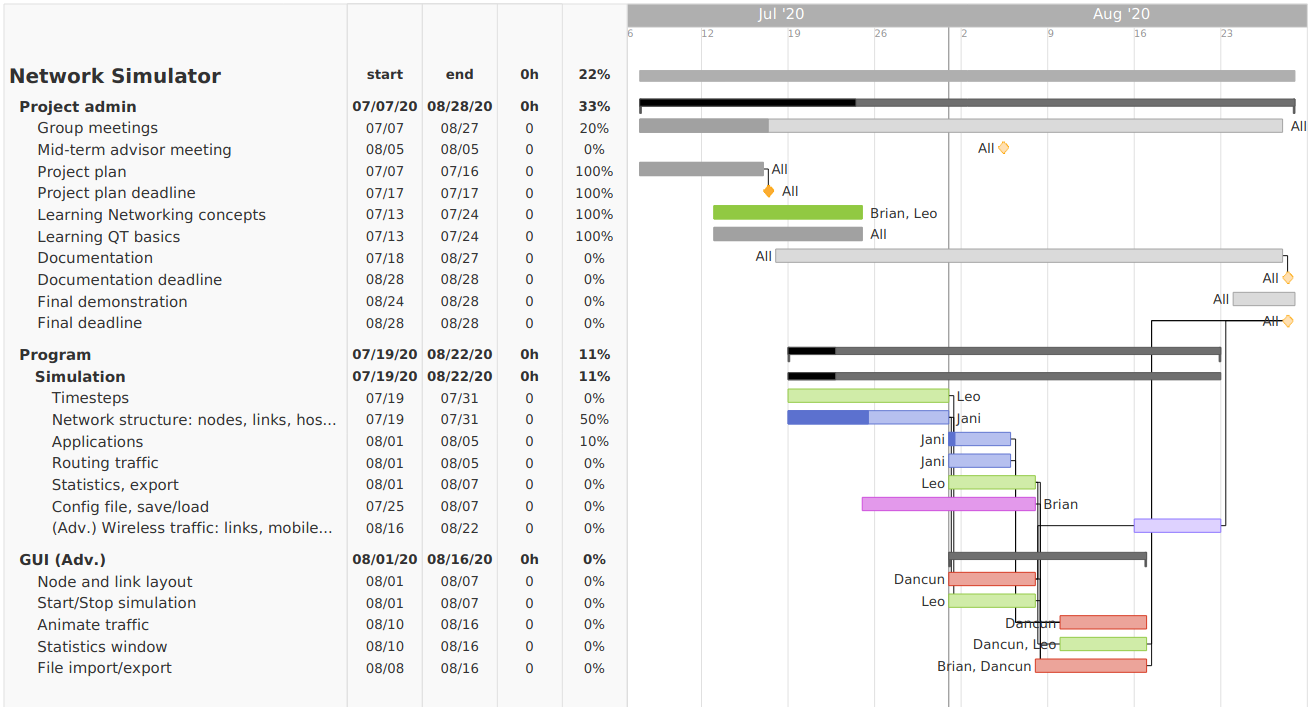
\includegraphics[width=13cm]{originalschedule.png}
    \caption{Original schedule from the project plan.}
	\label{img:schedule}			% use \ref{img:example} to refer to this figure
\end{center}
\end{figure}

The GUI was being worked on as mentioned, and some functionality was achieved:
% TODO Dancun
\begin{enumerate}
    \item \textcolor{red}{Dancun please write here about the GUI, some screenshots of what functionality you wrote already, some that was missing}
    \item Functionality 2
    \item Feature 3
\end{enumerate}

